% Chapter: 01_intro
% Included from lectures/slides.tex

\section{What is Mechanistic Interpretability?}

\begin{frame}[shrink=12]{Two Ways to Relate to Models}
\begin{columns}[T]
\begin{column}{0.48\textwidth}
\begin{center}
\textbf{\large Machine Learning}
\vspace{0.5em}

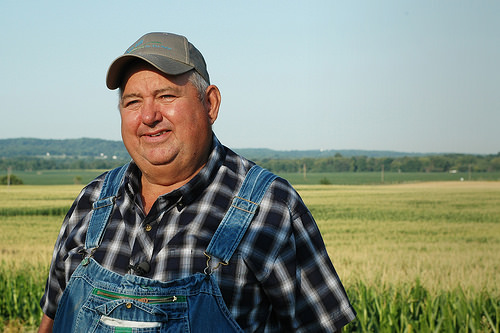
\includegraphics[width=0.75\textwidth]{figures/honest_work.jpg}
\end{center}

\begin{itemize}
\item Output-oriented
\item Find hyperparameters to improve models
\end{itemize}
\end{column}

\begin{column}{0.48\textwidth}
\begin{center}
\textbf{\large Mech.\ Interpretability}
\vspace{0.5em}

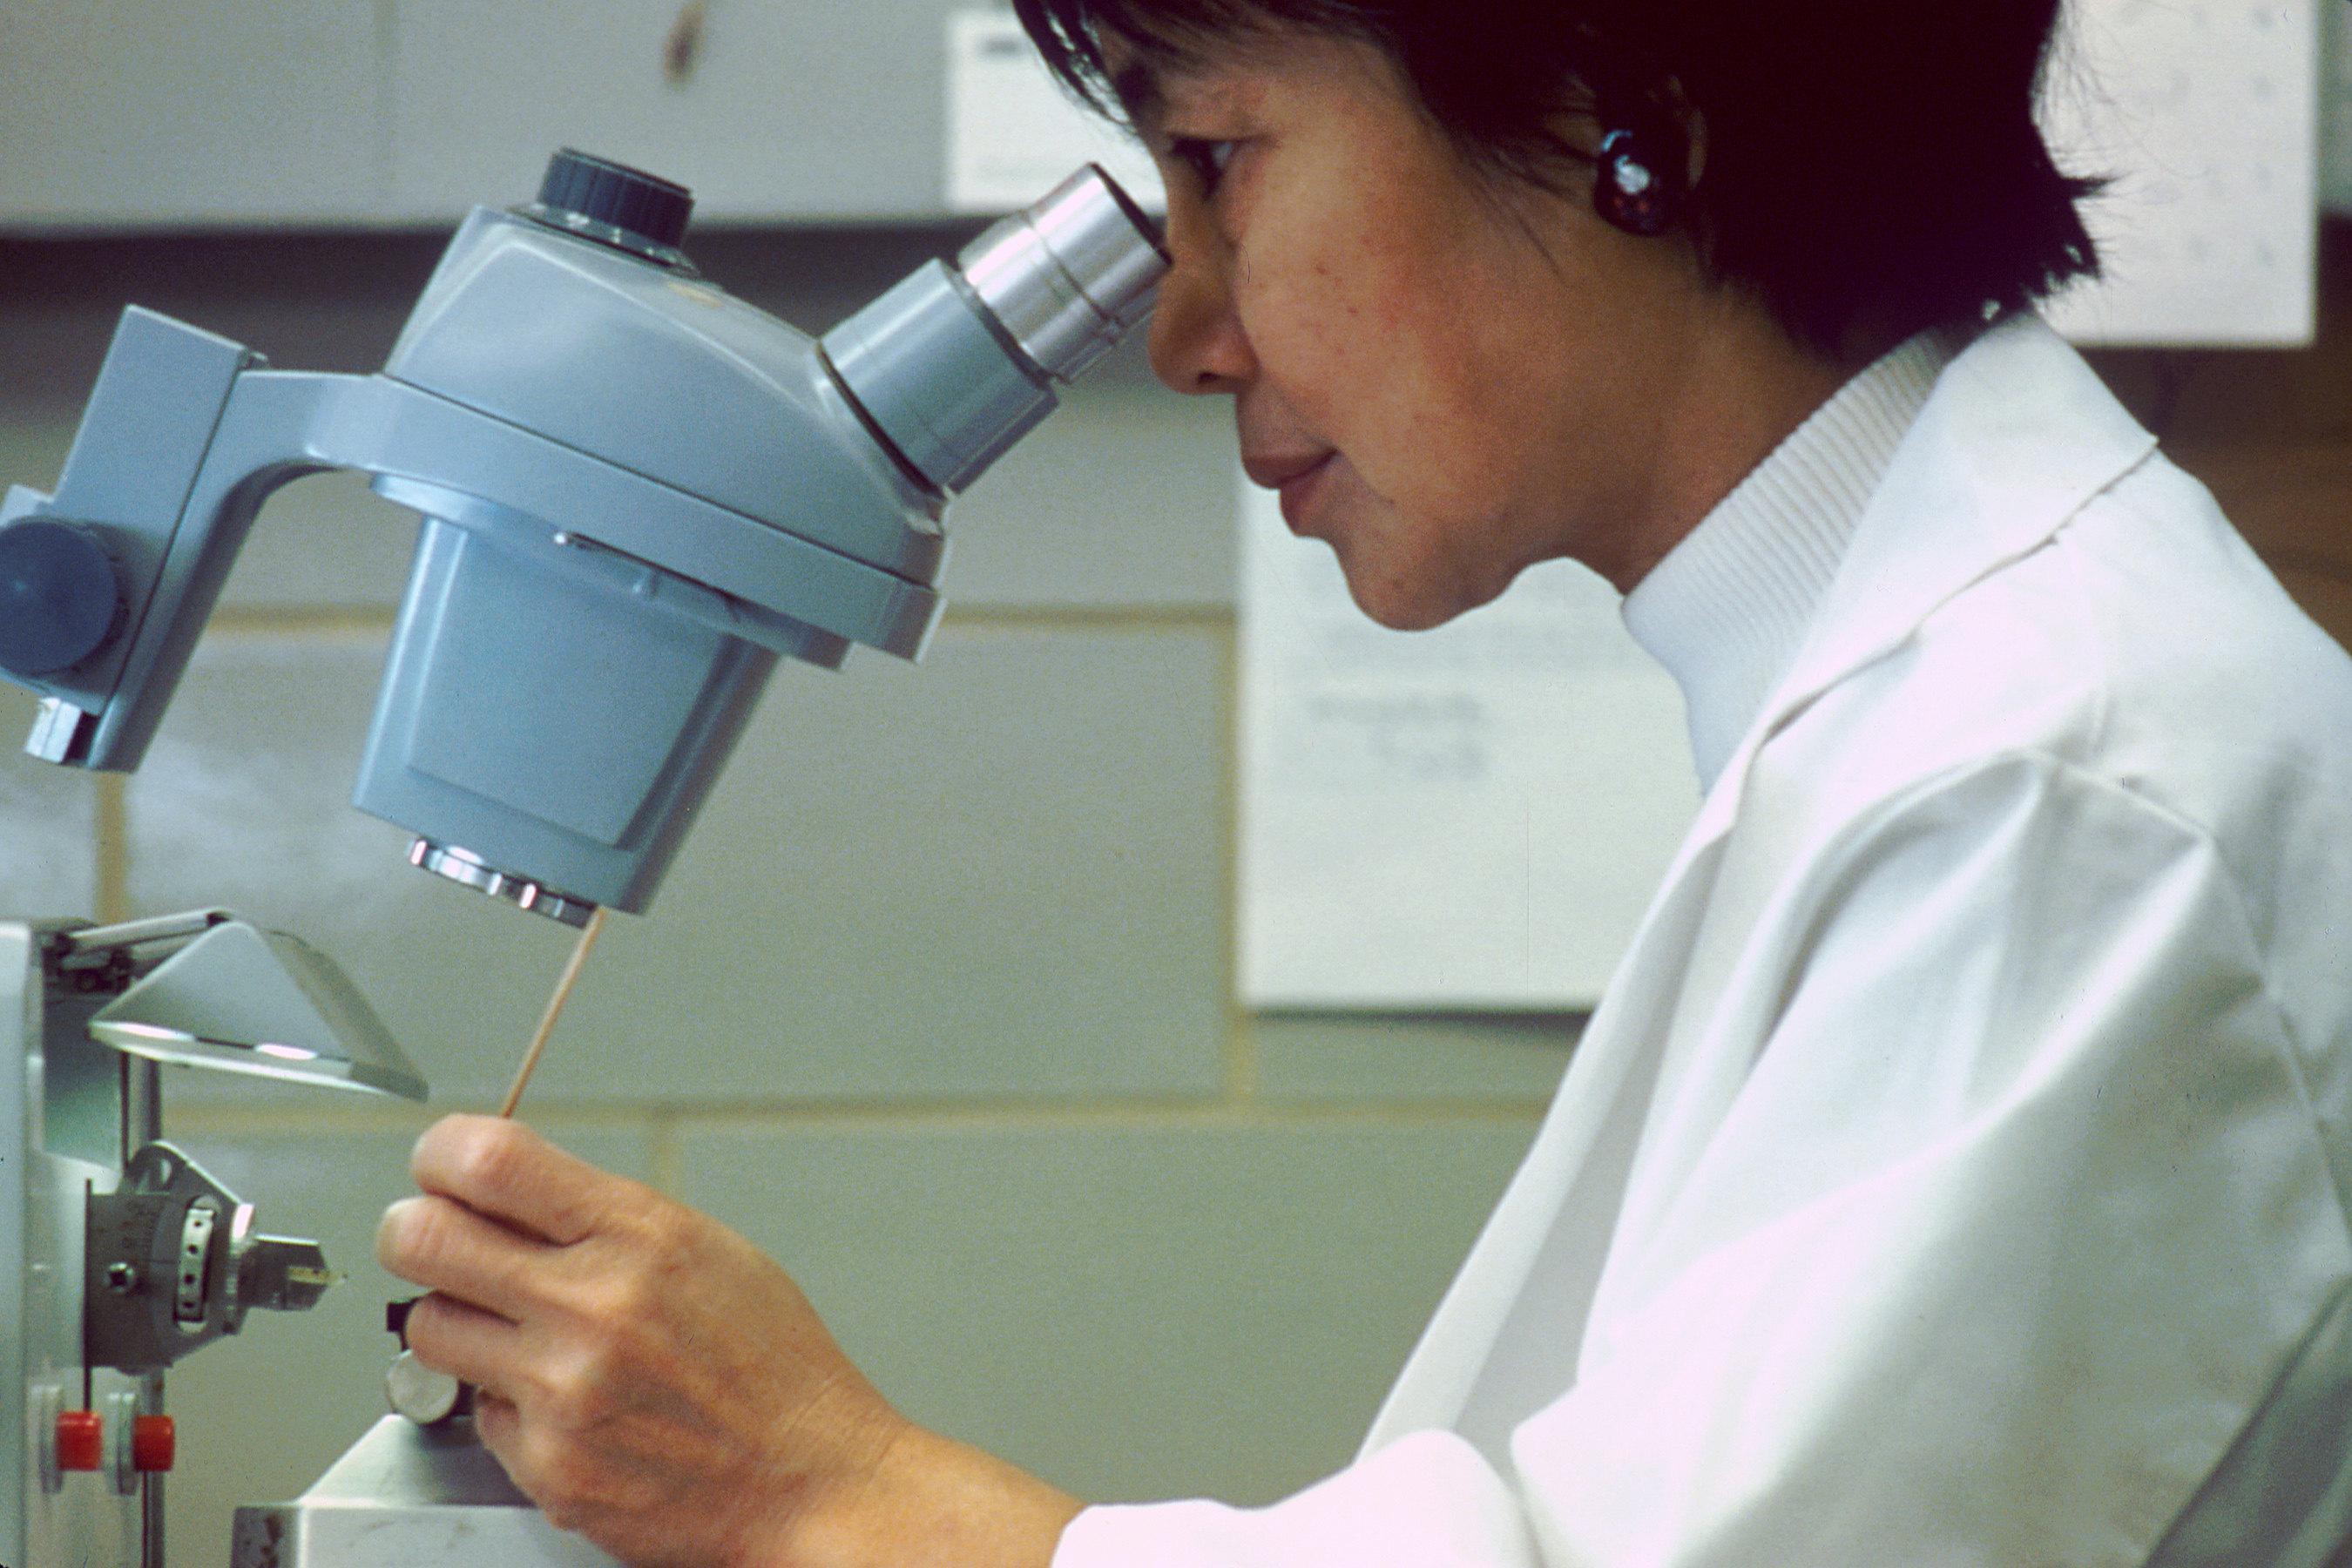
\includegraphics[width=0.75\textwidth]{figures/scientist_microscope.jpg}
\end{center}

\begin{itemize}
\item Learned models are the object of study
\item Understand and reverse-engineer parameters
\end{itemize}
\end{column}
\end{columns}

\note{
\begin{itemize}
\item Two ways to relate to neural networks
\item The standard ML view: models are tools, output is what matters, tune hyperparameters until they work
\item The mech interp view: the learned model is the object of study, treat it like a biologist treats an organism
\end{itemize}
}
\end{frame}

\begin{frame}[plain]
\vfill
\begin{center}
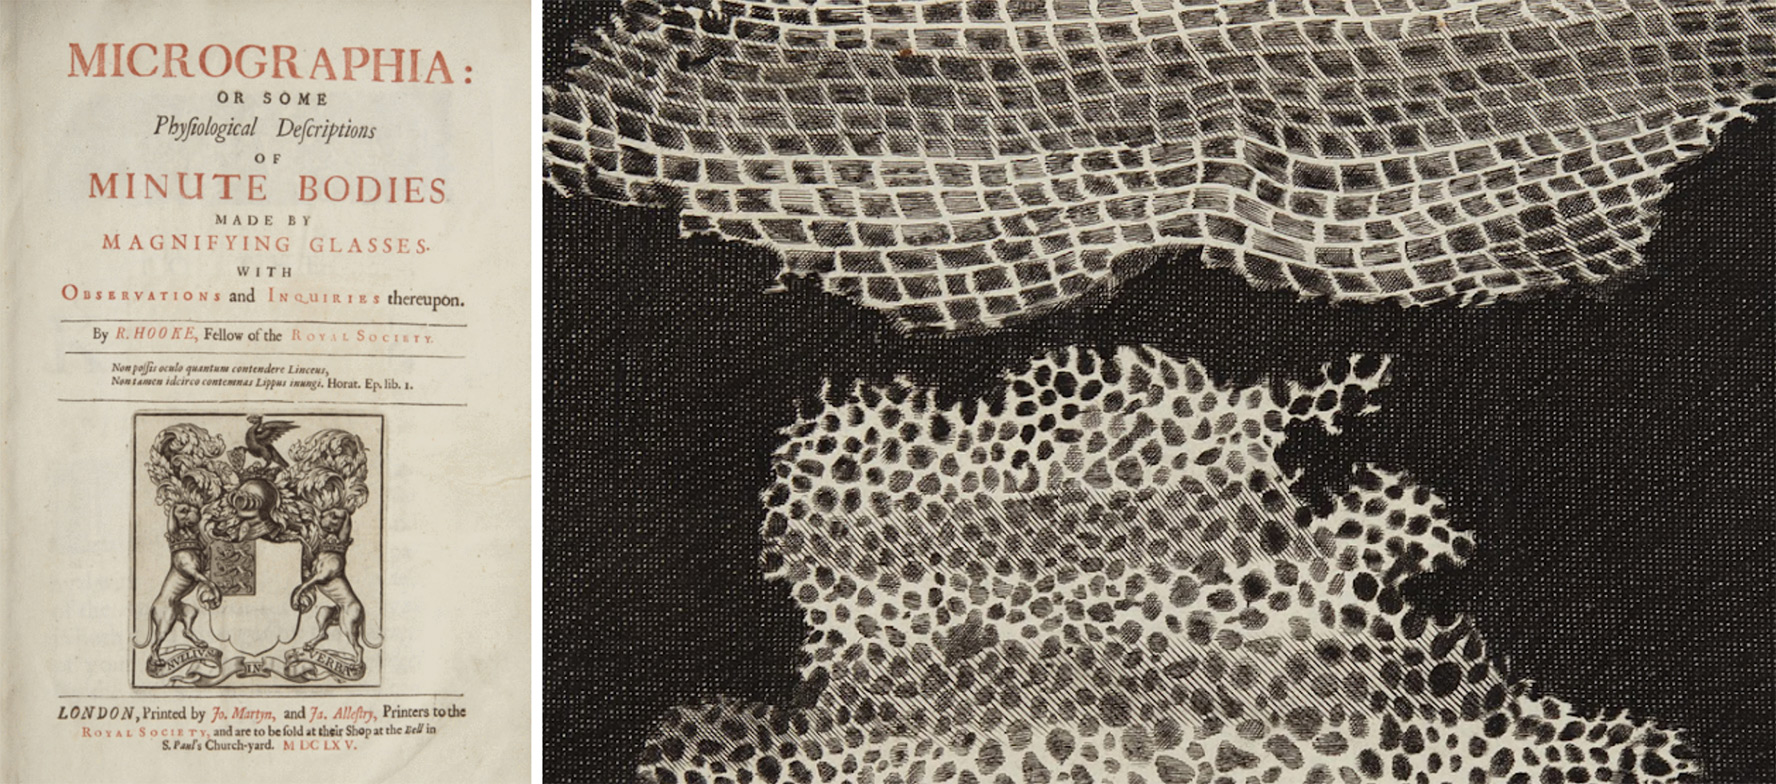
\includegraphics[width=\textwidth,height=0.9\textheight,keepaspectratio]{figures/micrographia.jpg}
\end{center}
\vfill
\source{olah2020}

\note{
\begin{itemize}
\item Normally in ML, we look at the algorithms we use to create neural networks: architectures, optimizers, hyperparameters, training data
\item We actively make decisions about these, so it makes sense to focus on them
\item Chris Olah's idea: look at the neural networks that come out of ML as objects of scientific inquiry
\item Similar to biologists not just studying evolution, but studying organisms by looking inside them
\item People tried to understand how life works for a long time
\item Ancient Greeks: the body is made of 4 humors that must be balanced
\item Doctors for centuries tried bloodletting and purging --- not crowned by success
\item The problem: wrong ontology. Understanding humors is not helpful for understanding disease
\item The right ontology came with the microscope: organisms are made of cells
\item Study cells, their properties, what makes them work, what bacteria cause which sicknesses --- then you get somewhere
\item Olah's vision: do for ML what the microscope did for biology
\end{itemize}
}
\end{frame}

\begin{frame}{Three Speculative Claims}
\begin{columns}[c]
\begin{column}{0.6\textwidth}
\begin{enumerate}
\item \textbf{Features} are the fundamental unit of neural networks.
They correspond to directions.
These features can be rigorously studied and understood.

\vspace{0.5em}
\item Features are connected by weights, forming \textbf{circuits}.
These circuits can also be rigorously studied and understood.

\vspace{0.5em}
\item \textbf{Universality}: Analogous features and circuits form across models and tasks.
\end{enumerate}
\end{column}
\begin{column}{0.35\textwidth}
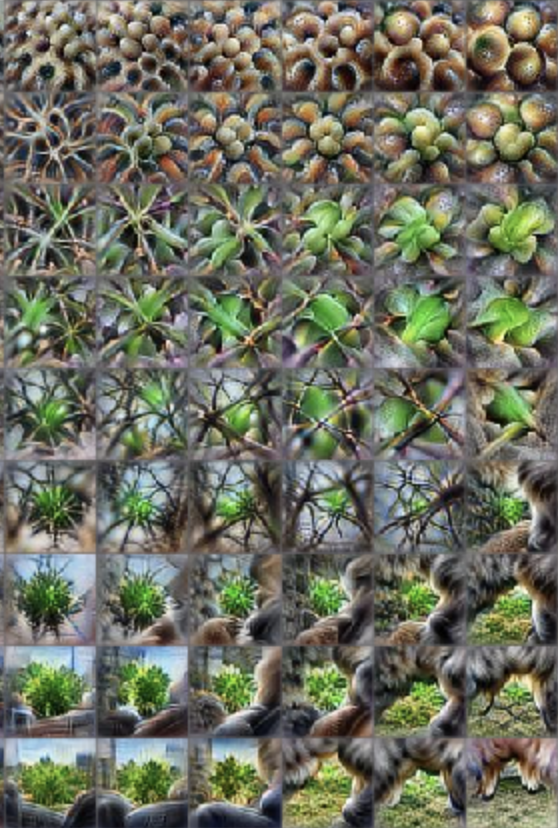
\includegraphics[width=\textwidth,height=0.8\textheight,keepaspectratio]{figures/activation_atlas_book.png}
\end{column}
\end{columns}

\source{olah2020}

\note{
\begin{itemize}
\item In his 2020 essay ``Zoom In'', Olah lays down similar claims to define a tentative ontology for MechInterp
\item These are not only descriptive, but normative
\item Claim 1: a feature is a fundamental unit, corresponding to a direction in activation space. The claim is that individual directions can be understood, and they are fundamental units
\item Question to audience: how would the world look if this claim were false? (possible: binary encoding, context-dependent meanings)
\item Claim 2: features connected by weights form circuits that can be understood
\item Question: what if Claim 1 is true but Claim 2 is false? (possible: features are readable storage but the process itself is more complicated, like CoT being readable but the LLM's use of it being inscrutable)
\item Claim 3: universality
\item If false: we could not learn from one network to another, every new NN would have completely different features and circuits
\end{itemize}
}
\end{frame}

\begin{frame}{}
\begin{center}
\Large How would MechInterp help AI safety?
\end{center}

\note{
\begin{itemize}
\item Now, what if those claims turn out to be true, how would that help with AI safety?
\item Question to audience, collecting ideas
\end{itemize}
}
\end{frame}

% \toicards{audit status}{enumerative status}{elk status}: theories of impact, optional traffic-light status line per card
\newcommand{\toicards}[3]{%
\begin{tikzpicture}[x=1cm,y=1cm]
\foreach \y in {0,0.55,1.1,1.65,2.2} \draw[fill=fb!15,draw=fb!50,rounded corners=2pt] (0,\y) rectangle (2.4,\y+0.4);
\node[font=\small\bfseries] at (1.2,3.0) {model internals};
\foreach \y/\ttl/\desc/\stat in {
  3.1/Auditing/{Find hidden goals or deception before deployment}/{#1},
  1.15/Enumerative safety/{List every feature, check that none is dangerous}/{#2},
  -0.85/Eliciting latent knowledge/{Read out what the model knows or believes}/{#3}} {
  \draw[-{Stealth[length=6pt]},thick,black!50] (2.6,1.3) -- (4.2,\y);
  \node[card,anchor=west,text width=7.6cm] at (4.3,\y) {\textbf{\ttl}\\\desc\ifx\relax\stat\relax\else\\[2pt]\stat\fi};
}
\end{tikzpicture}}

\begin{frame}{Theories of Impact}
\centering
\toicards{}{}{}

\source{nanda2022,elhage2022}

\note{
\begin{itemize}
\item Auditing: if we can find features/circuits for misaligned motivation, cheating, thinking about bioweapons, etc., we could detect this before or during deployment
\item Enumerative safety: if we can identify the function of every part of a neural network, we can be sure it does not contain bad intentions or dangerous capabilities
\item Eliciting latent knowledge: we can find out more directly what the model knows
\item Helps with transparency, against scheming
\item Also helps with ``AI for science'': e.g.\ a genetics model that knows some genetic marker is responsible for some effect, but since it is not a language model, you cannot just ask it
\item We come back to this slide at the end of the hour: how much of this does MechInterp deliver today?
\end{itemize}
}
\end{frame}

\begin{frame}{The Story of Today}
\centering
\begin{tikzpicture}[x=1cm,y=1cm,stage/.style={draw=fb!60,fill=fb!10,rounded corners=4pt,text width=2.35cm,minimum height=2.1cm,align=center,font=\footnotesize}]
\foreach \i/\ttl/\desc in {
  0/Neurons can mean things/{curve detectors, dog faces (vision models)},
  1/Concepts are directions/{read, add, and remove concepts},
  2/Too many concepts/{superposition, sparse autoencoders},
  3/Following the computation/{circuits, attribution graphs},
  4/Where it stands/{real-world uses, critiques}} {
  \node[stage] (s\i) at (\i*2.85,0) {\textbf{\ttl}\\[4pt]\textcolor{black!60}{\desc}};
}
\foreach \i [count=\j] in {0,...,3} \draw[-{Stealth[length=6pt]},thick,fb!60] (s\i) -- (s\j);
\end{tikzpicture}

\note{
\begin{itemize}
\item Roadmap for the first hour
\item We start where MechInterp started: vision models, where single neurons often mean something
\item Then language models: concepts live in directions, and we can read and edit them
\item Then the main complication (superposition) and the main tool against it (sparse autoencoders)
\item Then circuits: how features combine into computation
\item Finally: what is this used for today, and what are the critiques
\end{itemize}
}
\end{frame}
